% Slide 5 | Model and E3 | M5 (Saatwik Tiwari) | 2:00 | Bertram's bands and the daily-checking test
\begin{frame}{Bertram's optimal bands, and daily checking}
\framesubtitle{Slide 5 \textbullet\ Model and E3 \textbullet\ M5 \textbullet\ 2:00}
\vspace{-2pt}
\begin{columns}[T,onlytextwidth]
\column{0.49\textwidth}
  \small\raggedright
  One trade is a cycle: enter at $a$, exit at $m>a$, pay round-trip cost $c$.
  {\footnotesize\[ \mathbb{E}[T]=\frac{\pi}{\kappa}\Big[\erfi\!\Big(\tfrac{m\sqrt\kappa}{\sigma}\Big)-\erfi\!\Big(\tfrac{a\sqrt\kappa}{\sigma}\Big)\Big] \]
  \[ \mu(a,m)=\frac{m-a-c}{\mathbb{E}[T]} \]}
  \begin{itemize}\setlength{\itemsep}{2pt}
    \item symmetric bands $a=-m$: choose $m$ to maximise $\mu$
    \item a higher cost pushes the best band $m^*$ outwards
  \end{itemize}
\column{0.47\textwidth}
  \centering
  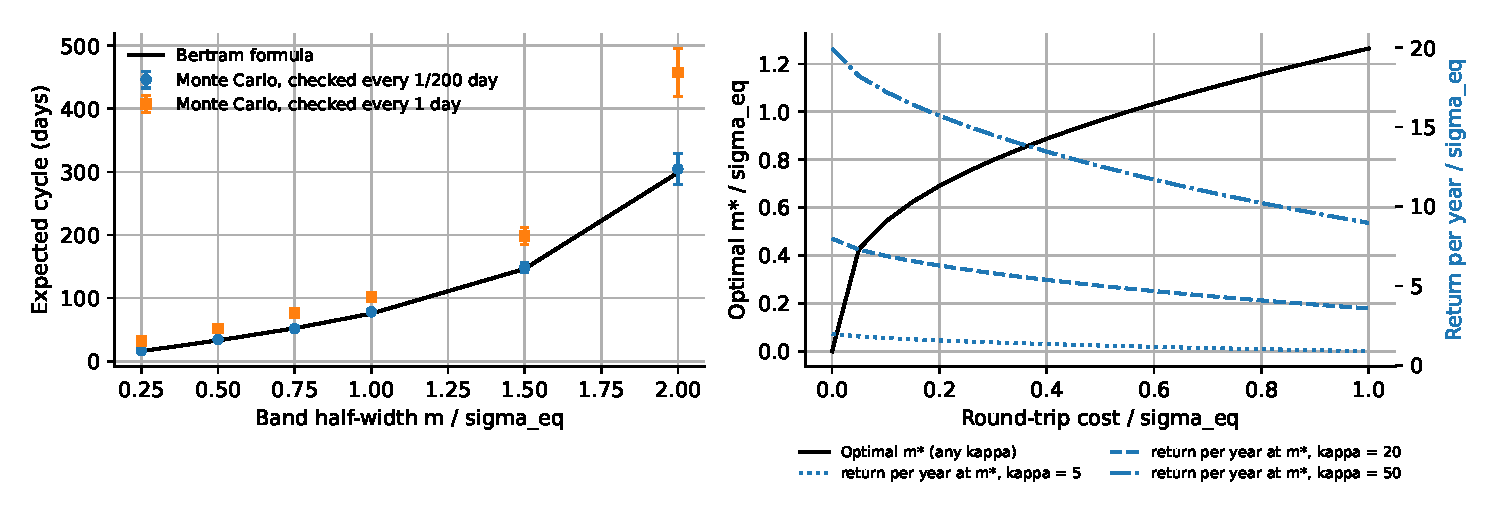
\includegraphics[width=\linewidth,trim=0bp 0bp 374bp 0bp,clip]{fig_e3_bertram}\\[2pt]
  \footnotesize\raggedright
  \textbf{E3:} the formula is \textbf{exact} (matches numerical integration to $10^{-8}$), but checking once a day makes a cycle \textbf{35--99\% longer}
\end{columns}
\pairTakeaway{The spread can cross a band and return between two daily looks.}
\end{frame}
